\chapter{Exemplos}
\label{cap:exemplos}

\section{Figuras}

A Figura~\ref{fig:exemplo} foi desenhada com TikZ. Para inserir uma imagem, coloque o
arquivo em \texttt{figuras/} e use \verb|\includegraphics{figuras/arquivo}|.

\begin{figure}[htb]
    \centering
    \caption{Exemplo de figura.}
    \label{fig:exemplo}
    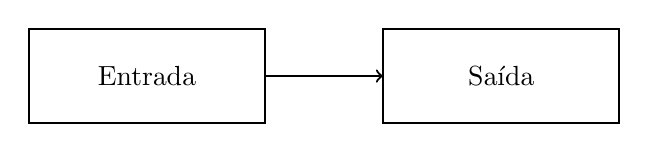
\begin{tikzpicture}
        \draw[thick] (0,0) rectangle (3,1.2) node[midway] {Entrada};
        \draw[->, thick] (3,0.6) -- (4.5,0.6);
        \draw[thick] (4.5,0) rectangle (7.5,1.2) node[midway] {Saída};
    \end{tikzpicture}
    \fonte{Elaborada pelo autor.}
\end{figure}

\section{Tabelas}

\begin{table}[htb]
    \centering
    \caption{Exemplo de tabela.}
    \label{tab:exemplo}
    \begin{tabular}{lcc}
        \toprule
        Método & Acurácia & F1 \\
        \midrule
        A & 0,81 & 0,79 \\
        B & \textbf{0,85} & \textbf{0,83} \\
        \bottomrule
    \end{tabular}
    \fonte{Elaborada pelo autor.}
\end{table}

\section{Equações e definições}

\begin{definicao}
    Uma definição numerada por capítulo.
\end{definicao}

\begin{equation}
    \mathcal{L} = -\sum_{i=1}^{n} y_i \log \hat{y}_i
    \label{eq:exemplo}
\end{equation}

A Equação~\eqref{eq:exemplo} é referenciada pelo seu rótulo.
